% mnras_template.tex
%
% LaTeX template for creating an MNRAS paper
%
% v3.0 released 14 May 2015
% (version numbers match those of mnras.cls)
%
% Copyright (C) Royal Astronomical Society 2015
% Authors:
% Keith T. Smith (Royal Astronomical Society)

% Change log
%
% v3.0 May 2015
%    Renamed to match the new package name
%    Version number matches mnras.cls
%    A few minor tweaks to wording
% v1.0 September 2013
%    Beta testing only - never publicly released
%    First version: a simple (ish) template for creating an MNRAS paper

%%%%%%%%%%%%%%%%%%%%%%%%%%%%%%%%%%%%%%%%%%%%%%%%%%
% Basic setup. Most papers should leave these options alone.
\documentclass[a4paper,fleqn,usenatbib]{mnras}

% MNRAS is set in Times font. If you don't have this installed (most LaTeX
% installations will be fine) or prefer the old Computer Modern fonts, comment
% out the following line
\usepackage{newtxtext,newtxmath}

% Depending on your LaTeX fonts installation, you might get better results with one of these:
%\usepackage{mathptmx}
%\usepackage{txfonts}

% Use vector fonts, so it zooms properly in on-screen viewing software
% Don't change these lines unless you know what you are doing
\usepackage[T1]{fontenc}
\usepackage{ae,aecompl}


%%%%% AUTHORS - PLACE YOUR OWN PACKAGES HERE %%%%%

% Only include extra packages if you really need them. Common packages are:
\usepackage{graphicx}	% Including figure files
\usepackage{amsmath}	% Advanced maths commands
\usepackage{amssymb}	% Extra maths symbols

\usepackage{xspace}

%%%%%%%%%%%%%%%%%%%%%%%%%%%%%%%%%%%%%%%%%%%%%%%%%%

%%%%% AUTHORS - PLACE YOUR OWN COMMANDS HERE %%%%%

% Please keep new commands to a minimum, and use \newcommand not \def to avoid
% overwriting existing commands. Example:
%\newcommand{\pcm}{\,cm$^{-2}$}	% per cm-squared

%%%%%%%%%%%%%%%%%%%%%%%%%%%%%%%%%%%%%%%%%%%%%%%%%%

\def\ngradeA{10}

\def\Sref#1{Section~\ref{#1}\xspace}
\def\Fref#1{Figure~\ref{#1}\xspace}
\def\Tref#1{Table~\ref{#1}\xspace}
\def\Eref#1{Equation~\ref{#1}\xspace}

\def\pr{{\rm Pr}}
\def\plens{\pr_{\mathrm{lens}}}

%%%%%%%%%%%%%%%%%%% TITLE PAGE %%%%%%%%%%%%%%%%%%%

% Title of the paper, and the short title which is used in the headers.
% Keep the title short and informative.
\title[]{SUGOHI I: automatic search for galaxy-galaxy strong lenses in the HSC survey}

% The list of authors, and the short list which is used in the headers.
% If you need two or more lines of authors, add an extra line using \newauthor
\author[A. Sonnenfeld et al.]{
Alessandro Sonnenfeld,$^{1}$\thanks{E-mail: alessandro.sonnenfeld@ipmu.jp}
Anupreeta More,$^{1}$
Masamune Oguri,$^{1,2}$
Yiping Shu,$^{3}$\newauthor
Sherry H. Suyu,$^{4}$
James H. H. Chan,$^{5}$
Kenneth C. Wong,$^{6}$
\\
% List of institutions
$^{1}$Kavli IPMU (WPI), UTIAS, The University of Tokyo, Kashiwa, Chiba 277-8583, Japan \\
$^{2}$Department of Physics, University of Tokyo, 7-3-1 Hongo, Bunkyo-ku, Tokyo 113-0033, Japan \\
$^{3}$National Astronomical Observatories, Chinese Academy of
Sciences, 20A Datun Road, Chaoyang District, Beijing 100012,
China \\
$^{4}$1Max-Planck-Institut fur Astrophysik, Karl-Schwarzschild-Str. 1, 85748 Garching, Germany \\
$^{5}$Department of Physics, National Taiwan University, 10617 Taipei, Taiwan
$^{6}$National Astronomical Observatory of Japan, 2-21-1 Osawa, Mitaka, Tokyo 181-8588, Japan
}
% These dates will be filled out by the publisher
\date{Accepted XXX. Received YYY; in original form ZZZ}

% Enter the current year, for the copyright statements etc.
\pubyear{2016}

% Don't change these lines
\begin{document}
\label{firstpage}
\pagerange{\pageref{firstpage}--\pageref{lastpage}}
\maketitle

% Abstract of the paper
\begin{abstract}
We developed a method to look for galaxy-scale strong gravitational lenses in photometric data. We applied it to the first internal data release of the HSC SSP survey. We found $\ngradeA$ definite lenses, Y probable lenses and Z possible lenses.
\end{abstract}

% Select between one and six entries from the list of approved keywords.
% Don't make up new ones.
\begin{keywords}
keyword1 -- keyword2 -- keyword3
\end{keywords}

%%%%%%%%%%%%%%%%%%%%%%%%%%%%%%%%%%%%%%%%%%%%%%%%%%

%%%%%%%%%%%%%%%%% BODY OF PAPER %%%%%%%%%%%%%%%%%%

\section{Introduction}

Lenses are great.

\section{The Data}

\subsection{HSC photometry}
The HSC survey is great.

\subsection{BOSS spectroscopy}
BOSS is great.

\section{The Method}

Method overview.

\subsection{Light subtraction}

\subsection{Lensed image identification}

\subsection{Foreground model}

\subsection{Lens model}

\subsection{Non-lens model}

\subsection{Tests on the SL2S sample}

\section{The photometrically selected sample}

\subsection{Candidate grading}
We graded lens candidates output by YattaLens according to their likelihood of being strong lenses, $\plens$, using the following scheme:
\begin{itemize}
\item Grade A: definite lenses ($\plens > 0.997$), 
\item Grade B: probable lenses ($0.5 < \plens < 0.997$)
\item Grade C: possible lenses ($0.003 < \plens < 0.5$)
\item Grade 0: non lenses ($plens < 0.003$)
\end{itemize}

\section{The spectroscopically selected sample}

\section{Results}
In \Fref{fig:gradeA} we show the grade A lenses.
%
\begin{figure*}
 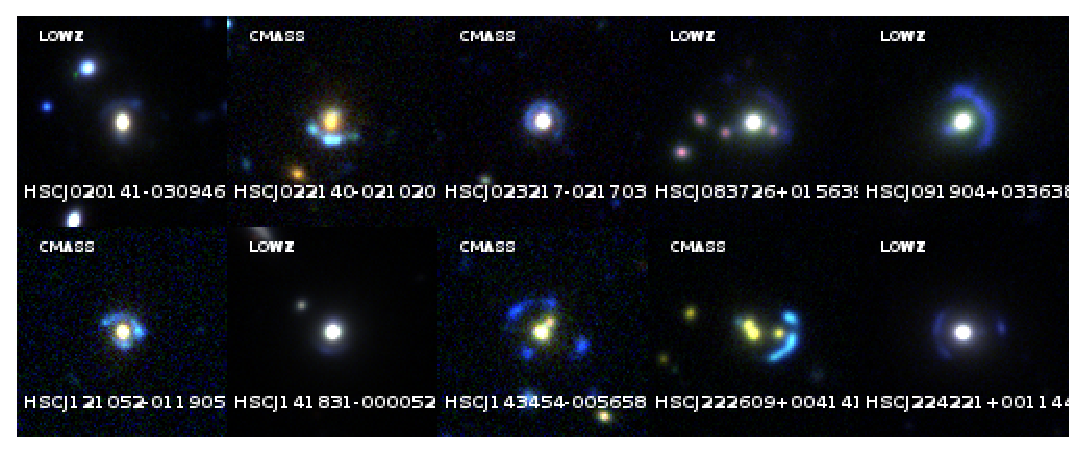
\includegraphics[width=\textwidth]{gradeA_collage.eps}
 \caption{Grade A lenses.}
 \label{fig:gradeA}
\end{figure*}
%
\section{Discussion}

\subsection{Lenses missed by YattaLens}

\subsection{Comparison with other lens samples}

\section{Conclusions}

\section*{Acknowledgements}

Acknowledgements.

%%%%%%%%%%%%%%%%%%%%%%%%%%%%%%%%%%%%%%%%%%%%%%%%%%

%%%%%%%%%%%%%%%%%%%% REFERENCES %%%%%%%%%%%%%%%%%%

% The best way to enter references is to use BibTeX:

%\bibliographystyle{mnras}
%\bibliography{example} % if your bibtex file is called example.bib


% Alternatively you could enter them by hand, like this:
% This method is tedious and prone to error if you have lots of references
\begin{thebibliography}{99}
\bibitem[\protect\citeauthoryear{Author}{2012}]{Author2012}
Author A.~N., 2013, Journal of Improbable Astronomy, 1, 1
\bibitem[\protect\citeauthoryear{Others}{2013}]{Others2013}
Others S., 2012, Journal of Interesting Stuff, 17, 198
\end{thebibliography}

%%%%%%%%%%%%%%%%%%%%%%%%%%%%%%%%%%%%%%%%%%%%%%%%%%

%%%%%%%%%%%%%%%%% APPENDICES %%%%%%%%%%%%%%%%%%%%%

\appendix

\section{Some extra material}

If you want to present additional material which would interrupt the flow of the main paper,
it can be placed in an Appendix which appears after the list of references.

%%%%%%%%%%%%%%%%%%%%%%%%%%%%%%%%%%%%%%%%%%%%%%%%%%


% Don't change these lines
\bsp	% typesetting comment
\label{lastpage}
\end{document}

% End of mnras_template.tex
